\section{Regler-Entwurf}
\begin{tcolorbox}[colback=white!10!white,colframe=green!30!black] 

	\begin{enumerate}
		\item 	Die Zustandsrückführung ist : $u = -\bs{Kx}$ einsetzen in $\dot{\bs{x}} = \bs{Fx}+\bs{G}u$
		\item $\dot{\bs{x}} = (\bs{F}-\bs{GK})\bs{x}$
		\item Für vorgegebene Pole $s_i$ charakteristische Gleichung aufstellen
		\item $\det (s\bs{I}-\bs{F}+\bs{GK})$ ergibt die charakteristische Gleichung in Abhängigkeit von $\bs{K} = \begin{bmatrix}
		k_1 & \ldots & kn
		\end{bmatrix}$
		\item Koeffizentenvergleich zwischen beiden charakteristischen Gleichungen $\Rightarrow \bs{K}$ 
	\end{enumerate} 
\tcblower
\textbf{System in Regelungsnormalform}
$K$ ist besonders einfach, wenn ein System in RNF vorliegt.
\begin{align*}
	\bs{A}_C-\bs{B}_C\bs{K} = \begin{bmatrix}
	0 & 1& 0&\ldots&0\\ 	0 & 0& 1&\ldots&0\\
	0 & 0& 0&\ddots&0\\
	0 & 0& 0&\ldots&1\\
	-a_n-k_1 & -a_{n-1}-k_2& &\ldots&-a_{1}-k_n\\
	\end{bmatrix}
\end{align*}
Die charakteristische Gleichung ergibt sich sofort zu:
\begin{align*}
	s^n +(a_1+k_n)s^{n-1}+(a_2+k_{n-1})s^{n-2}+\ldots+(a_n+k_1) =0 
\end{align*}

Man kann direkt den Koeffizientenvergleich machen - Determinantenbildung entfällt.
	
\end{tcolorbox}

\begin{tcolorbox}[colback=white!10!white,colframe=green!30!black,title=Integralregelung]
	Charakteristische Gleichung $0=det(s\bs{I}-\bs{A}_a+\bs{B}_a*\bs{K})$
	Integralregelung  sorgt dafür der Fehler bei Änderung der Streckenparameter Null wird. Das System wir um einen Integralen Teil erweitert.
	\begin{align*}
		\begin{bmatrix}
		\dot{	\bs{x}_I} \\ \dot{	\bs{x}}
		\end{bmatrix} &= \begin{bmatrix}
		0 & \bs{H} \\ 0 & \bs{F}
		\end{bmatrix}\begin{bmatrix}
			\bs{x}_I \\	\bs{x}
		\end{bmatrix}+
		\begin{bmatrix}
		0 \\ \bs{G}
		\end{bmatrix} u - \begin{bmatrix}
		1 \\ 0
		\end{bmatrix}r
	\end{align*}
	mit dem Regler:
	\begin{align*}
		u = -\begin{bmatrix}
		 K_1 & \bs{K_0}
		\end{bmatrix} \begin{bmatrix}
			\bs{x}_I \\\bs{x}
		\end{bmatrix} = - \bs{K} \begin{bmatrix}
		\bs{x}_I \\\bs{x}
		\end{bmatrix}
	\end{align*}
	
	\begin{figure}[H]
\centering
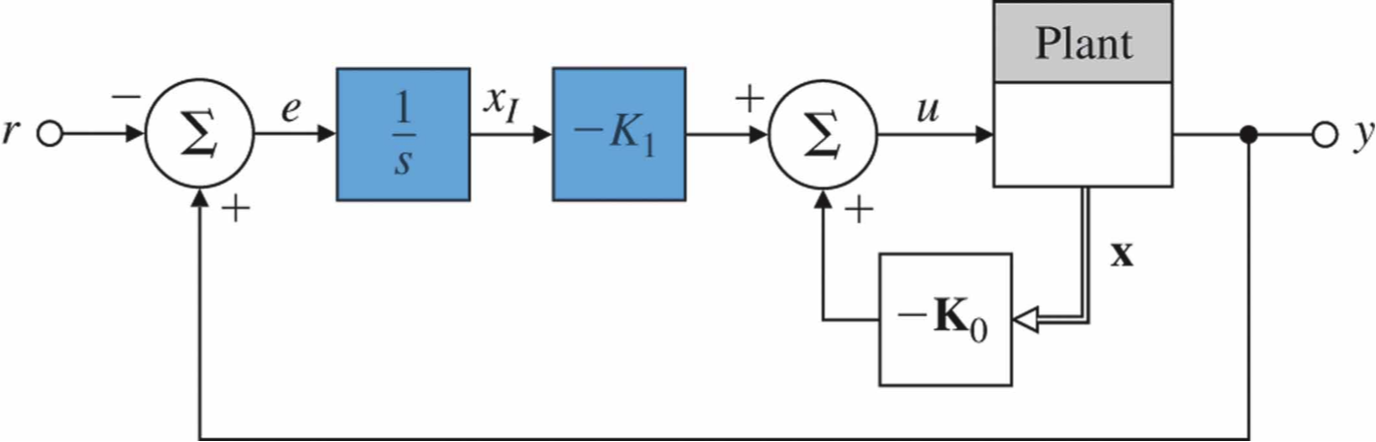
\includegraphics[width=0.7\linewidth]{content/img/integral}

\end{figure}
\tcblower
\textbf{Beispiel:}
Übertragungsfunktion $\frac{Y(s)}{U(s)} = \frac{1}{s+3}$\\
Systembeschreibung $F = -3, G = 1, H = 1$

Gewünscht Pole bei $s=-5$ + Integralanteil \\$\Rightarrow a_C(s) = s^2+10s+25$

Die erweiterte Systembeschreibung ergibt sich zu:
\begin{align*}
		\begin{bmatrix}
		\dot{	\bs{x}_I} \\ \dot{	\bs{x}}
		\end{bmatrix} = \begin{bmatrix}
			0 & 1\\ 0 & -3
		\end{bmatrix} \begin{bmatrix}
		\bs{x}_I \\\bs{x}
		\end{bmatrix} + \begin{bmatrix}
		0 \\1
		\end{bmatrix}u - \begin{bmatrix}
		1\\0
		\end{bmatrix}r
\end{align*}
Die Rückführmatrix 
\begin{align*}
	&\det\left( s\bs{I} - \begin{bmatrix}
	0 & 1\\ 0 & -3
	\end{bmatrix}+ \begin{bmatrix}
	0 \\1
	\end{bmatrix}\bs{K}\right) \overset{!}{=} s^2 +10s +25\\
	&\bs{K} = \begin{bmatrix}
		K_1 & K_2
	\end{bmatrix} = \begin{bmatrix}
	25 & 7
	\end{bmatrix}
\end{align*}
\end{tcolorbox}